%----------------------------------------------------------------------------
\chapter{Helyreállítás tesztelése}
%----------------------------------------------------------------------------

Ebben a fejezetben két jeleneten tesztelem a helyreállítás minőségét. Az elsőben a két kamerát egymás mellé helyezem úgy, hogy képsíkjaik nagyjából egybeessenek, míg a második jelenetnél a két kamera optikai tengelye egy hegyes szöget zár be.

A teszteléshez két darab Logitech QuickCam Pro 9000 típusú webkamerát használtam, melyektől VGA felbontású ($640\times 480$) képeket kértem le.

% -------------------------------------------------------
\section{Első jelenet}
% -------------------------------------------------------

Elsőként egy olyan jeleneten próbáltam ki az elkészült alkalmazást, amely esetén a két kamera egymás mellett van (lásd \ref{fig:scene1_camerapose}. ábra), egy irányba néznek, és két teás dobozt mozgatok előttük. A jelenet 178 képkockából állt (\textasciitilde 6 másodperc), melyből mindegyik $640\times 480$-as felbontású, színes kép. \Aref{fig:scene1_frames}. ábrán látható a bal oldali kamerák által rögzített 3 képkocka és -- a könnyebb összehasonlíthatóság végett -- ugyanezen nézőpontból vett helyreállításaival együtt. Megfigyelhető, hogy a bal oldali teás doboz rekonstrukciója a textúrázatlan területeken várakozásainknak megfelelően hiányos, hiszen itt nem hagyatkozhattunk az optikai folyam által adódó elmozdulásokra. Ugyanezen okok miatt a szereplő kezeiből is csak néhány pontot lehetett helyreállítani.

\begin{figure}[tbh]
\centering
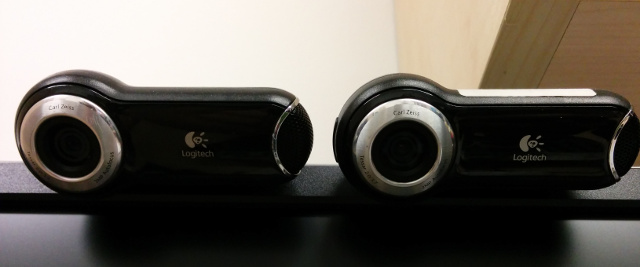
\includegraphics[width=300pt]{figures/scene1_camerapose.jpg}
\caption{Kamerák helyzete az első jelenetnél \label{fig:scene1_camerapose}}
\end{figure}

\begin{figure}[tbh]
\centering
\begin{subfigure}[b]{.32\linewidth}
	\centering
	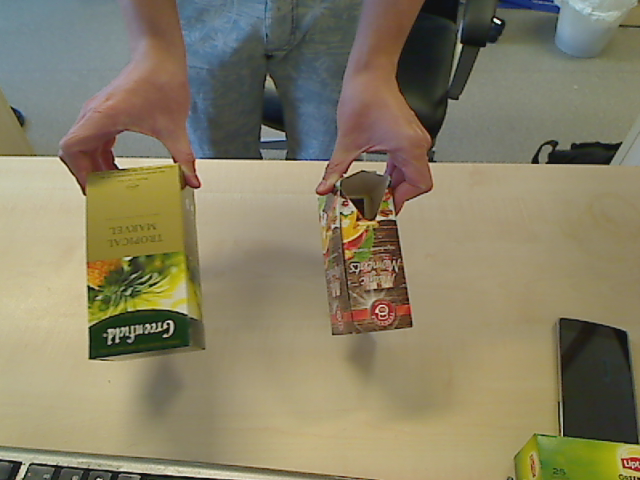
\includegraphics[width=135pt]{figures/left_93.png}
  \end{subfigure}
\begin{subfigure}[b]{.32\linewidth}
	\centering
	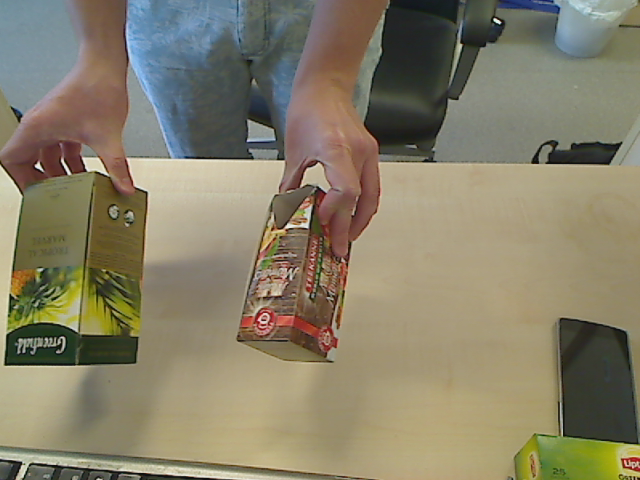
\includegraphics[width=135pt]{figures/left_153.png}
  \end{subfigure}
\begin{subfigure}[b]{.32\linewidth}
	\centering
	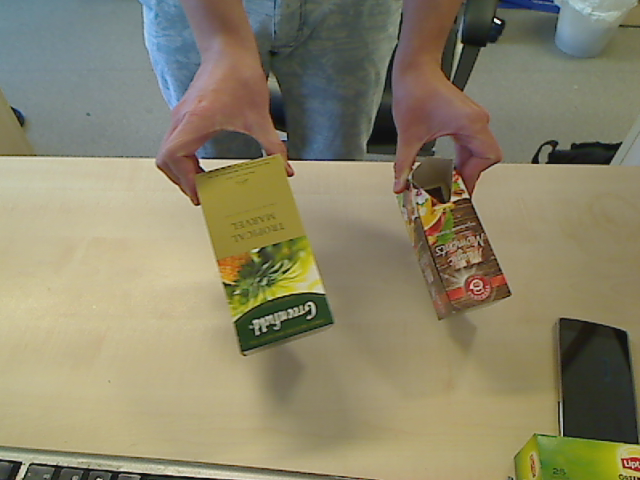
\includegraphics[width=135pt]{figures/left_223.png}
  \end{subfigure}\\\vspace{5pt}
\begin{subfigure}[b]{.32\linewidth}
	\centering
	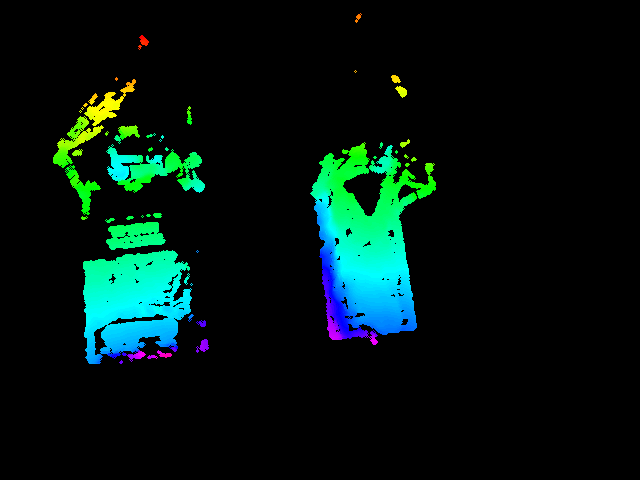
\includegraphics[width=135pt]{figures/vis_93.png}
  \end{subfigure}
\begin{subfigure}[b]{.32\linewidth}
	\centering
	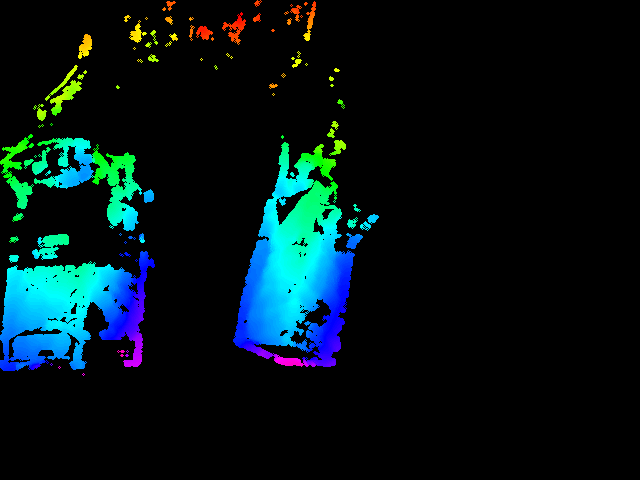
\includegraphics[width=135pt]{figures/vis_153.png}
  \end{subfigure}
\begin{subfigure}[b]{.32\linewidth}
	\centering
	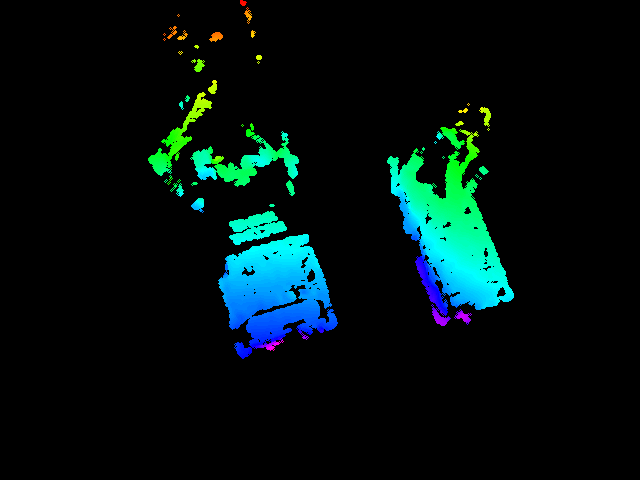
\includegraphics[width=135pt]{figures/vis_223.png}
  \end{subfigure}
\caption{A bal oldali kamera 3 képkockája (40., 100. és 170. képkocka) az első jelenetből, valamint a helyreállított képek a baloldali kamera nézőpontjából \label{fig:scene1_frames}}
\end{figure}

A 178 képkockából 157-szer kaptam \aref{fig:scene1_frames}. ábrához hasonló rekonstrukciókat, 13-szor csak 1 objektumot sikerült helyreállítani, illetve 8-szor volt értékelhetetlen a végeredmény (nagyon kicsi pontfelhő, néhány ponttal). A hibák akkor történtek, amikor a jelenetben a két doboz nem mozgott jelentősen, csak helyben forgott, minek következtében az előtér maszkok hiányosak lettek. A rekonstrukciók során az összes képkockára nézve az átlagos pixel visszavetítési hiba 0,8 lett, ami elhanyagolhatónak számít. A már bemutatott pillanatokhoz rajzolt kontúrok \aref{fig:scene1_contours}. ábrán látható. Megfigyelhető, hogy a jobb oldali doboz pusztán kontúrja alapján is felismerhető, viszont a bal oldai doboz textúrázottságának hiánya jelentősen befolyásolja a kontúrjainak értelmezhetőségét.

\begin{figure}[tbh]
\centering
\begin{subfigure}[b]{.32\linewidth}
	\centering
	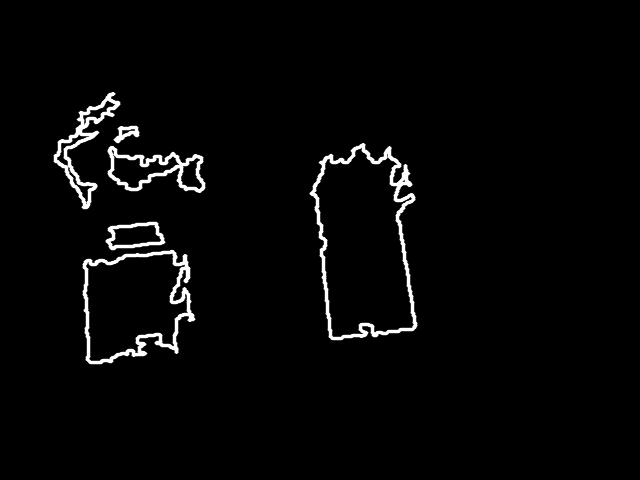
\includegraphics[width=135pt]{figures/contour_93.png}
  \end{subfigure}
\begin{subfigure}[b]{.32\linewidth}
	\centering
	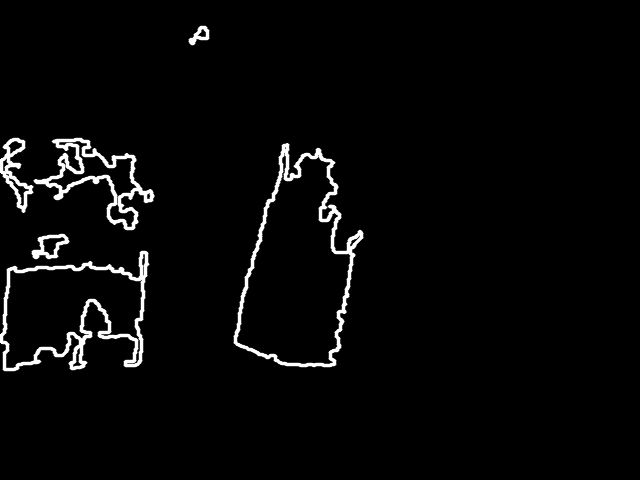
\includegraphics[width=135pt]{figures/contour_153.png}
  \end{subfigure}
\begin{subfigure}[b]{.32\linewidth}
	\centering
	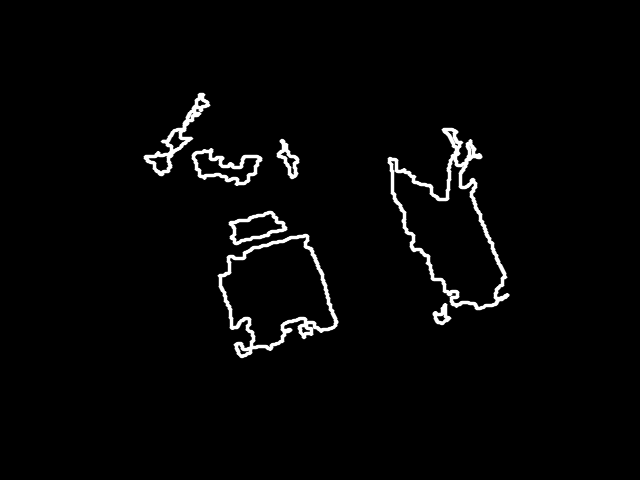
\includegraphics[width=135pt]{figures/contour_223.png}
  \end{subfigure}
\caption{A 40., 100. és 170. képkockák alapján számolt kontúrok a baloldali kamera nézőpontjából \label{fig:scene1_contours}}
\end{figure}

% -------------------------------------------------------
\section{Második jelenet}
% -------------------------------------------------------

Második jelenet két olyan kamera által került rögzítésre, amelyek optikai tengelyei egy hegyes szöveg zárnak be (lásd \ref{fig:scene2_camerapose}. ábra). Ebben az esetben is a jelenetben két teás dobozt mozgattam. A jelenet 360 képkockából állt (\textasciitilde 12 másodperc), melyből mindegyik $640\times 480$-as felbontású, színes kép. \Aref{fig:scene2_frames}. ábrán látható a bal oldali kamerák által rögzített 4 képkocka és ugyanezen nézőpontból vett helyreállítások vizualizációi.

\begin{figure}[b!]
\centering
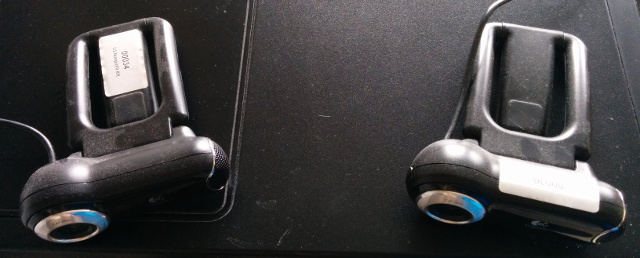
\includegraphics[width=280pt]{figures/scene2_camerapose.jpg}
\caption{Kamerák helyzete a második jelenetnél \label{fig:scene2_camerapose}}
\vspace{15pt}
\begin{subfigure}[b]{.32\linewidth}
	\centering
	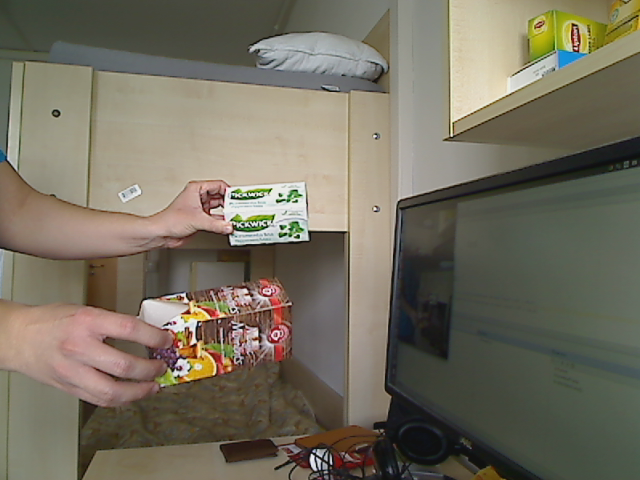
\includegraphics[width=135pt]{figures/scene2/left_45.png}
  \end{subfigure}
\begin{subfigure}[b]{.32\linewidth}
	\centering
	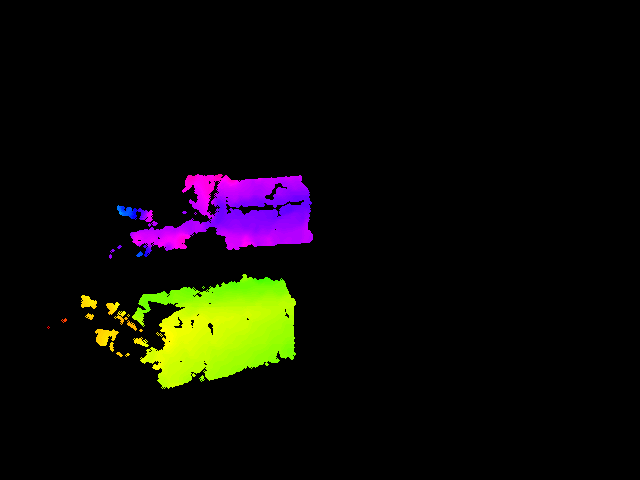
\includegraphics[width=135pt]{figures/scene2/vis_45.png}
  \end{subfigure}
\begin{subfigure}[b]{.32\linewidth}
	\centering
	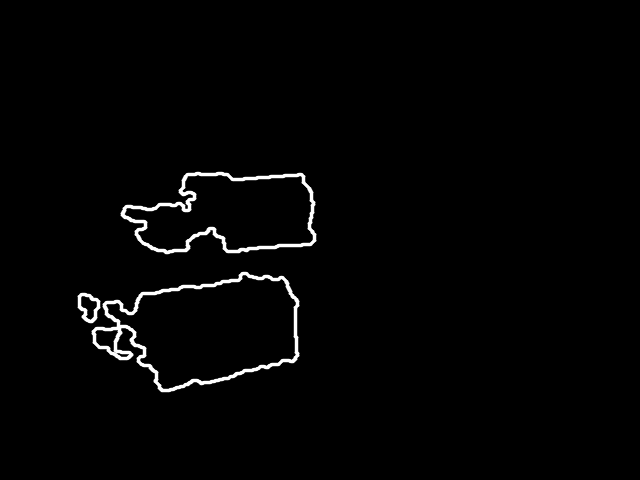
\includegraphics[width=135pt]{figures/scene2/ctr_45.png}
  \end{subfigure}\\\vspace{5pt}
  \begin{subfigure}[b]{.32\linewidth}
	\centering
	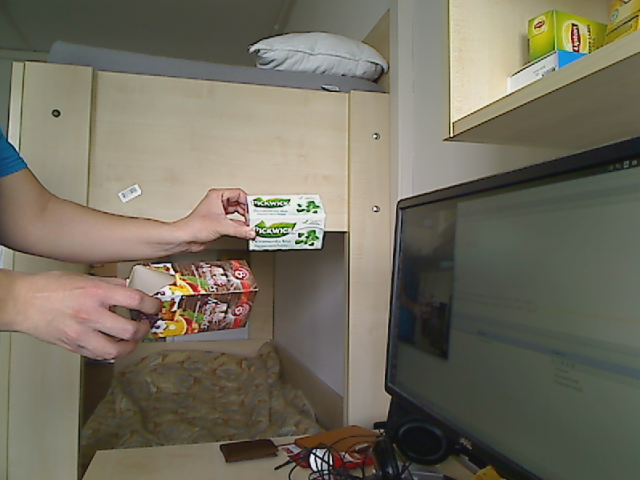
\includegraphics[width=135pt]{figures/scene2/left_130.png}
  \end{subfigure}
\begin{subfigure}[b]{.32\linewidth}
	\centering
	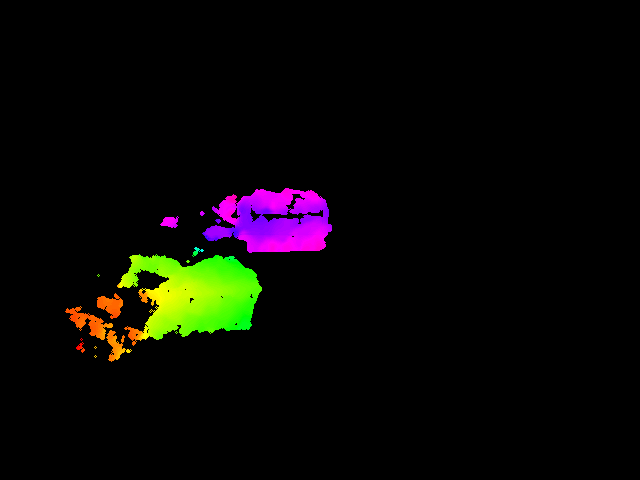
\includegraphics[width=135pt]{figures/scene2/vis_130.png}
  \end{subfigure}
\begin{subfigure}[b]{.32\linewidth}
	\centering
	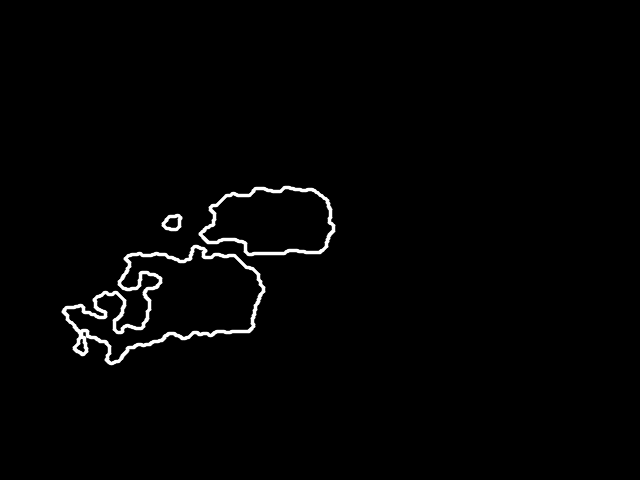
\includegraphics[width=135pt]{figures/scene2/ctr_130.png}
  \end{subfigure}\\\vspace{5pt}
  \begin{subfigure}[b]{.32\linewidth}
	\centering
	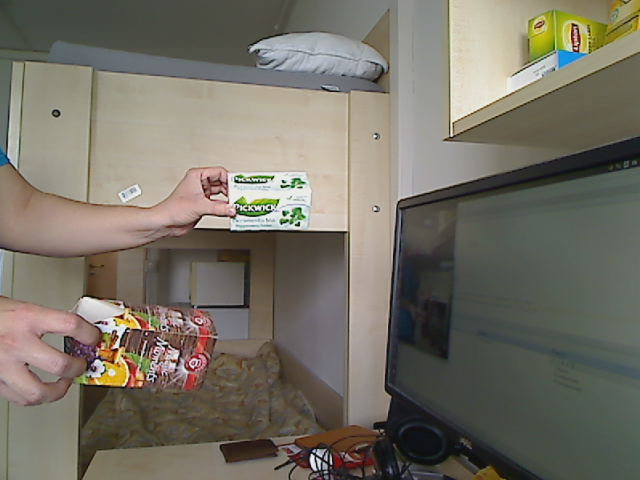
\includegraphics[width=135pt]{figures/scene2/left_215.png}
  \end{subfigure}
\begin{subfigure}[b]{.32\linewidth}
	\centering
	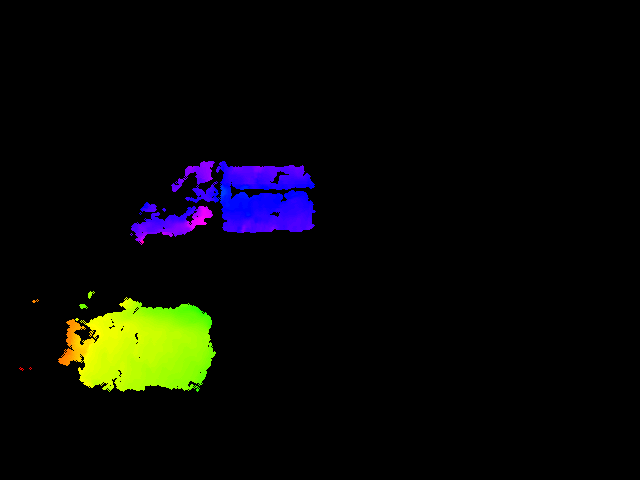
\includegraphics[width=135pt]{figures/scene2/vis_215.png}
  \end{subfigure}
\begin{subfigure}[b]{.32\linewidth}
	\centering
	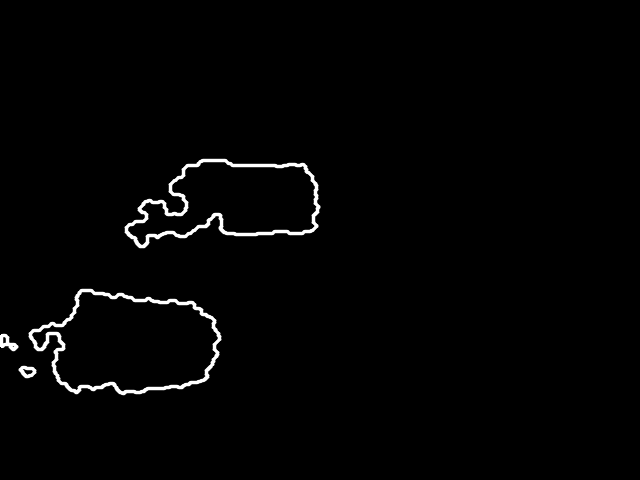
\includegraphics[width=135pt]{figures/scene2/ctr_215.png}
  \end{subfigure}\\\vspace{5pt}
  \begin{subfigure}[b]{.32\linewidth}
	\centering
	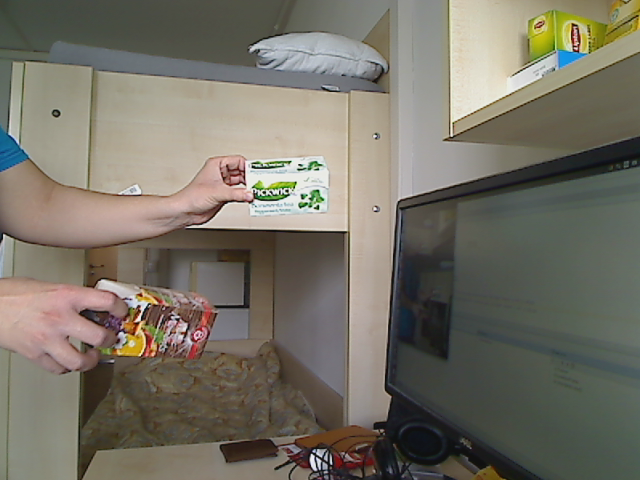
\includegraphics[width=135pt]{figures/scene2/left_339.png}
  \end{subfigure}
\begin{subfigure}[b]{.32\linewidth}
	\centering
	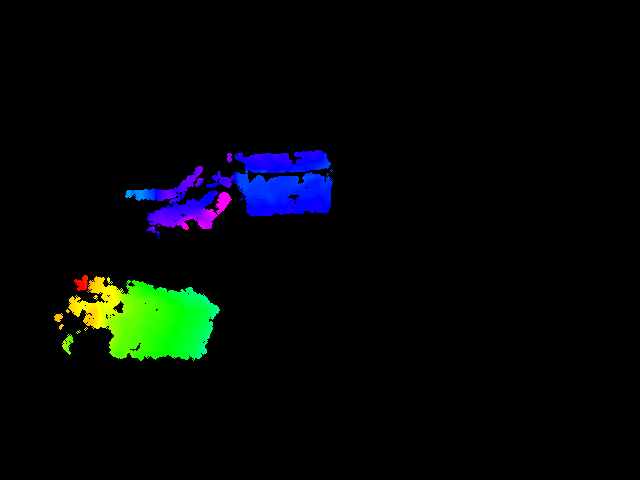
\includegraphics[width=135pt]{figures/scene2/vis_339.png}
  \end{subfigure}
\begin{subfigure}[b]{.32\linewidth}
	\centering
	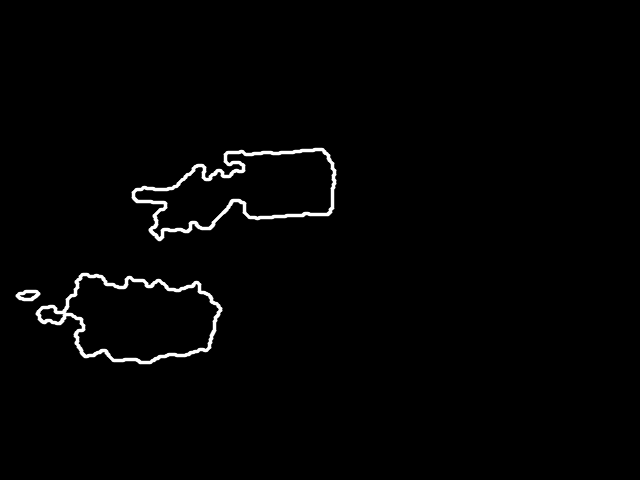
\includegraphics[width=135pt]{figures/scene2/ctr_339.png}
  \end{subfigure}
\caption{A második jelenethez tartozó 45., 130., 215. és 340. képkockák bal oldali képei és azok vizualizációi \label{fig:scene2_frames}}

\end{figure}

\begin{figure}[tbh]
\centering
\end{figure}

A képek jól mutatják, hogy elég sok pontot sikerült helyreállítani köszönhetően a jól textúrázott dobozoknak, lassú mozgásnak és a megfelelő fényviszoknak. Az átlagos visszavetítési hiba ennél a jelenetnél 1,5 pixel lett.

\Aref{fig:scene2_close}. ábrán látható két olyan helyzet, amikor a két doboz nagyon közel van egymáshoz. Az első esetben a hátul lévő dobozt szinte teljesen elveszítjük, míg a második esetben egész jól elkülönül térben az eredmény. Ekkor viszont a képen látható közelség miatt az előtér maszkok egybemosódnak, így egy objektumként fogja értelmezni őket, amit a kontúrrajzon is látható.

\begin{figure}[tbh]
\centering
\begin{tikzpicture}[spy using outlines={white,chamfered rectangle, magnification=1.5, width=2cm, height=1.5cm, connect spies}]

\node (A) {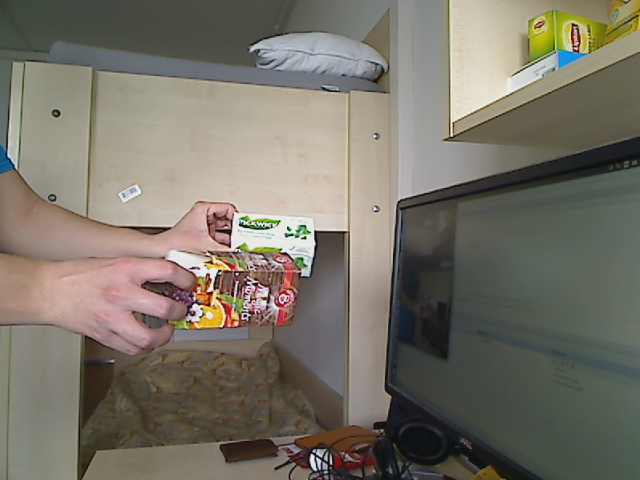
\includegraphics[width=135pt]{figures/scene2/left_182.png}};
%\spy on (-0.6,-0.2) in node [left] at (2.3,0.95);

\node (B) [right of=A,xshift=10.5em] {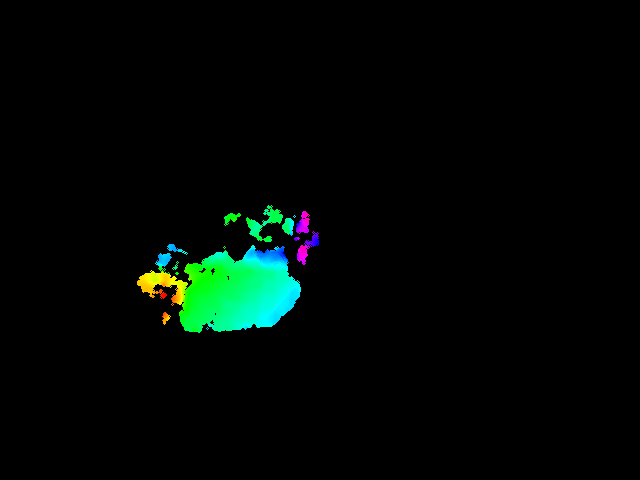
\includegraphics[width=135pt]{figures/scene2/vis_182.png}};

%\spy on ($(-0.6,-0.2)+(13.1em,0)$) in node [left] at ($(2.3,0.95)+(13.1em,0)$);

\node (C) [right of=B,xshift=10.5em] {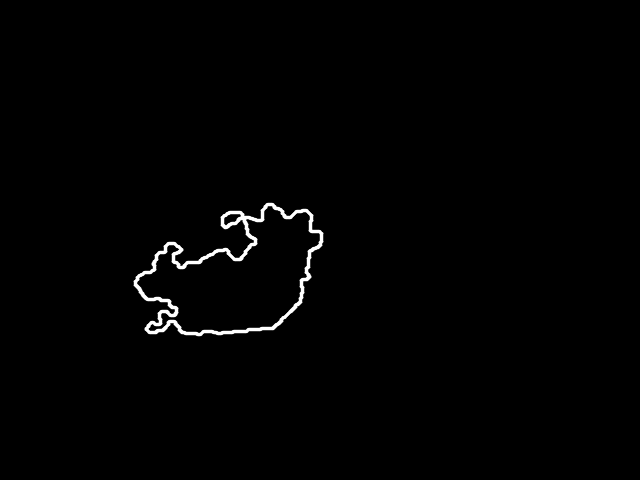
\includegraphics[width=135pt]{figures/scene2/ctr_182.png}};


\end{tikzpicture}\\\vspace{3pt}

\begin{tikzpicture}[spy using outlines={white,chamfered rectangle, magnification=1.5, width=2.1cm, height=1.7cm, connect spies}]

\node (A) {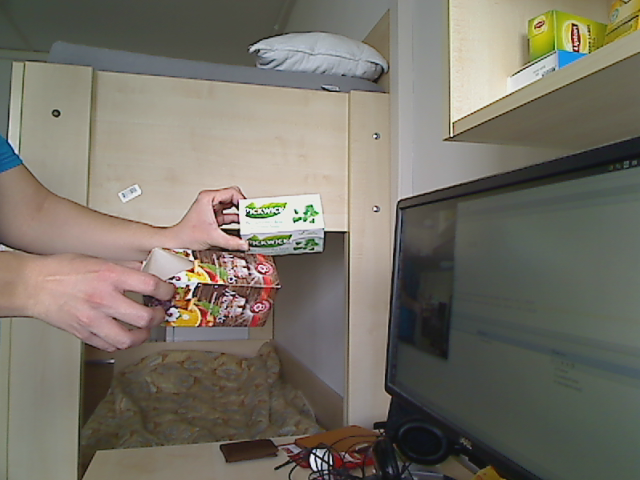
\includegraphics[width=135pt]{figures/scene2/left_192.png}};
%\spy on (-0.6,-0.17) in node [left] at (2.3,-0.95);

\node (B) [right of=A,xshift=10.5em] {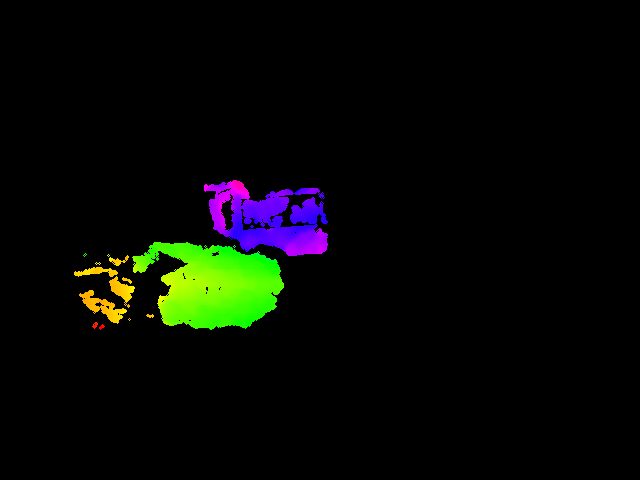
\includegraphics[width=135pt]{figures/scene2/vis_192.png}};

%\spy on ($(-0.6,-0.17)+(13.1em,0)$) in node [left] at ($(2.3,-0.95)+(13.1em,0)$);

\node (C) [right of=B,xshift=10.5em] {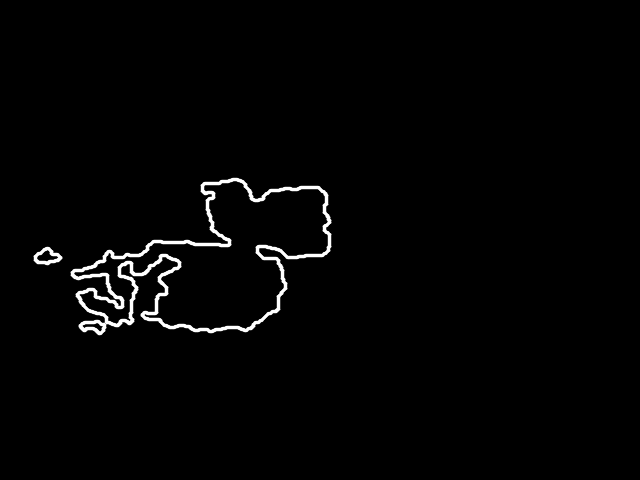
\includegraphics[width=135pt]{figures/scene2/ctr_192.png}};

\end{tikzpicture}

\caption{Amikor a két doboz közel van egymáshoz, kiemelve a részleteket \label{fig:scene2_close}}
\end{figure}

A két jelenet alapján nyugodtan állítható, hogy amennyiben eleget teszünk azon követelményeknek, miszerint az objektumok mozogjanak a képeken és a felületük textúrája ne legyen nagy felületeken egybefüggően homogén, akkor igen pontos és jól felismerhető rekonstrukciókat kapunk az elkészült megoldás segítségével.
